\normalfont


\documentclass[10pt,conference,letterpaper]{IEEEtran}
\usepackage[pdftex]{graphicx}
\usepackage{graphicx}
\usepackage[table]{xcolor}
\usepackage{booktabs}
\usepackage{tabularx}
\usepackage{balance}
\usepackage{makecell}
\usepackage{array}
\usepackage{cite}
\usepackage{hyperref} % for the url and hyperref
\usepackage{url}
\usepackage{float}
\usepackage{wrapfig}

\IEEEoverridecommandlockouts

\begin{document}

\bstctlcite{bstctl:etal}

\title{LLMMMM: Large Language Models Matrix-Matrix Multiplications Characterization on Open Source Silicon}

\author{\IEEEauthorblockN{Louis Ledoux\IEEEauthorrefmark{1}\IEEEauthorrefmark{2},
Marc Casas\IEEEauthorrefmark{1}\IEEEauthorrefmark{2}
}
\IEEEauthorblockA{\IEEEauthorrefmark{1}Barcelona Supercomputing Center, Barcelona, Spain}
\IEEEauthorblockA{\IEEEauthorrefmark{2}Universitat Polit\`ecnica de Catalunya, Barcelona, Spain}

E-mail: \{louis.ledoux,marc.casas\}@bsc.es\\

}

\maketitle

%ABSTRACT - Dis-comment the following lines to add an abstract
%\begin{abstract}
%You can add an abstract here
%\end{abstract}

\begin{keywords}
	Large Language Models (LLM), Transformers, Generative Pre-Trained (GPT), Matrix-Matrix Multiplications, Floating-Points, arithmetic, ASIC, Open-Source
\end{keywords}

\vspace{-4mm}
%%%%%%%%%%%%%%%%%%%%%%%%%%%%%%%%%%%%%%%%%%%%%%%%%%%%%%%%%%%%%%%%%%%%%%%%%%%%%%%
%%% Introduction
%%%%%%%%%%%%%%%%%%%%%%%%%%%%%%%%%%%%%%%%%%%%%%%%%%%%%%%%%%%%%%%%%%%%%%%%%%%%%%%
\section{Extended Abstract}
%\subsection{Introduction}
%\label{sec:introduction}
%
%GPT transformers are usefol for ..
%
%However, they cost a lot Prior work show the cost of~\cite{luccioni2022estimating}
%
%Esentially MMM, wity hdatya movement of datum, the arithmetic weigts etc.. (describe the matrices, number of elements)
%
%Recent work focus on designing Specialized format and algorithm to reduce the cost (reducing bitwdith, MLX, tpu, bitnet, ternary, 40\% layer remove)
%
%We introduce a generator of ASIC kernels agnostic to the PDK of MMM units of emerging and small floating point formnats, we then evaluate such units.

\subsection{Introduction}
\label{sec:introduction}

GPT transformers are useful for various applications, offering significant advancements in natural language processing tasks.
However, their operational costs are substantial has shown in prior work which highlights the financial implications of deploying these models~\cite{luccioni2022estimating}.

Essentially, matrix-matrix multiplications (MMM), with their intensive data movement and manipulation of arithmetic weights, underscore the computational demands of these architectures.
Naturally, these observations are also found in recent efforts within the research community, which have concentrated on devising specialized formats and algorithms aimed at mitigating these costs.
These innovations include reducing bit-width exemplified by Machine Learning eXchange (MLX) formats (essentially small floats)~\cite{}, specialized hardware such as TPUs' systolic arrays~\cite{}, model pruning of up to 40\%~\cite{}, and more recently, ternary and binary LLMs (see BitNets~\cite{}).

We introduce a generator of ASIC kernels agnostic to the PDK of MMM units for emerging and small floating-point formats, followed by the evaluation of such units.
Concretely, our contributions include the automated generation of circuits for any floating-point format with automated pipelining, a systolic array architecture proposal—these two combined form the foundation of MMM units, a framework to automate the translation from high-level language (Python) to silicon for such matrices (SUF, SuperSet Framework~\cite{}), the generation of $7 \text{ arithmetic formats} \times 2 \text{ accumulator configurations} \times 4 \text{ PDKs} = 56$ chips, and their performance and efficiency evaluation, all provided as open source.

\subsection{Biography}
\label{sec:biography}

\begin{wrapfigure}{l}{0.2\textwidth} % "l" for left and "0.25\textwidth" for the width of the wrap figure area
\centering
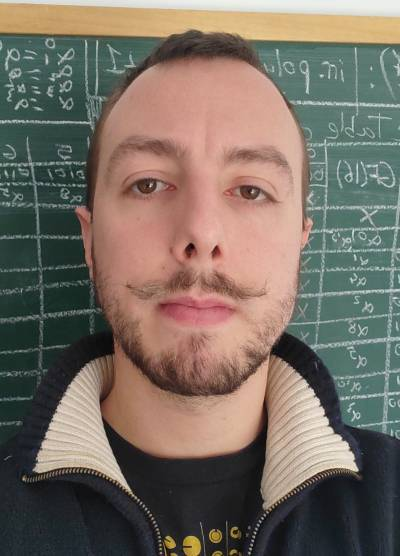
\includegraphics[width=0.18\textwidth]{./figures/louis2.jpg}
\end{wrapfigure}
Louis Ledoux, originating from a comprehensive computer science background in Rennes (Bretagne, France), has transitioned towards a hardware focus. His journey began with a Bachelor's degree, followed by a Master's in Computer Science, culminating in a one-year internship in 2017, where he explored FPGA virtualization in the cloud. Since 2018, Louis has been engaged in a PhD in computer arithmetic at the Universitat Polit\`ecnica de Catalunya and the Barcelona Supercomputing Center, in Barcelona, Spain. His main focus are hardware implementations to address numerical requirements sparsity in HPC workloads. Beyond academia, Louis contributes to the open hardware community, participating in efabless/skywater/Google tapeouts.

%\begin{figure}[H]
%\begin{minipage}[b]{0.1\linewidth}
%\centering
%	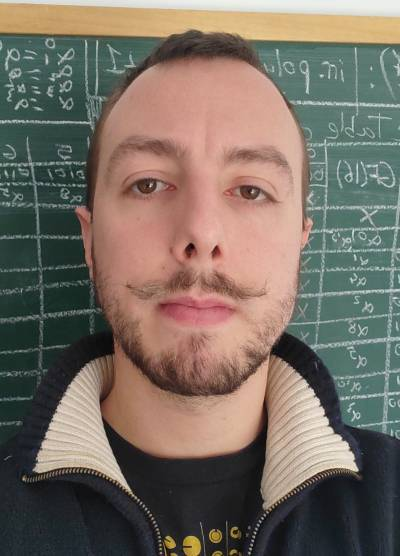
\includegraphics[width=\textwidth]{./figures/louis2.jpg}
%\end{minipage}
%\hspace{0.5cm}
%\begin{minipage}[b]{0.85\linewidth}
%\centering
%Louis Ledoux, originating from a comprehensive computer science background in Rennes (Bretagne, France), has transitioned towards a hardware focus.
%His journey began with a Bachelor's degree, followed by a Master's in Computer Science, culminating in a one-year internship in 2017, where he explored FPGA virtualization in the cloud.
%Since 2018, Louis has been engaged in a PhD in computer arithmetic at the Universitat Polit\`ecnica de Catalunya and Barcelona Supercomputing Center, in Barcelona, Spain.
%His main focus are hardware implementations to address numerical requirements sparsity in HPC workloads.
%Beyond academia, Louis contributes to the open hardware community, participating in efabless/skywater/Google tapeouts.
%\end{minipage}
%\end{figure}

\section{Acknowledgment}
\label{sec:acknowledgment}
Marc Casas has been partially supported by the Grant RYC-2017-23269 funded by MCIN/AEI/10.13039/501100011033 and by ESF Investing in your future. This research was supported by grant PID2019-107255GB-C21 funded by MCIN/AEI/ 10.13039/501100011033. Els autors agraeixen el suport del Departament de Recerca i Universitats de la Generalitat de Catalunya al Grup de Recerca "Performance understanding, analysis, and simulation/emulation of novel architectures" (Codi: 2021 SGR 00865).


\IEEEpeerreviewmaketitle

\vspace{-2mm}


\vspace{-2mm}

%%%%%%%%% -- BIB STYLE AND FILE -- %%%%%%%%
\balance
\bibliographystyle{IEEEtran}
%\bibliography{IEEEabrv,paper}

\bibliography{references.bib}
\vspace{-7mm}
%%%%%%%%%%%%%%%%%%%%%%%%%%%%%%%%%%%%

\end{document}
